% Options here are passed to the article class.
% Most common options: 10pt, 11pt, 12pt
\documentclass[10pt]{datasheet}

% Input encoding and typographical rules for English language
\usepackage[utf8]{inputenc}
\usepackage[english]{babel}
\usepackage[english]{isodate}

% tikz is used to draw images in this example, but you can
% also use \includegraphics{}.
\usepackage{graphicx}

% These define global texts that are used in headers and titles.
\title{DH02: Quad Display Slice With Passive Read}
\author{Obi, 51 mayday, and hampter}
\tags{display-halls, quad-display, slice, passive-read}
\date{December 2022}
\revision{Revision 1}

\begin{document}
\maketitle

\section{Features}

\begin{itemize}
\item{4 box displays \& chests per slice.}
\item{Minimum hoppers \& chests for this layout. Fully hopper locked.}
\item{In slice lists for which chests need to be restocked from empty.}
\item{Easily reachable \& visible inventories.}
\item{Control logic can be relatively simple.}
\end{itemize}

\section{Applications}

\begin{itemize}
\item{Encoded quad-display hall}
\end{itemize}

\section{General Description}
The DH02 quad display slice has 4 box displays with passive read ability. It has a fully hopperlocked layout with no visible pistons. The bottom displays has one buffer box with global first box placement. For full hopperlocking, the top displays require a gap every 32 blocks. Box collection is not fully reliable. Top display will break if used aggressively.
% Switch to next column
\vfill\break

\begin{figure}[h]
    \centering
    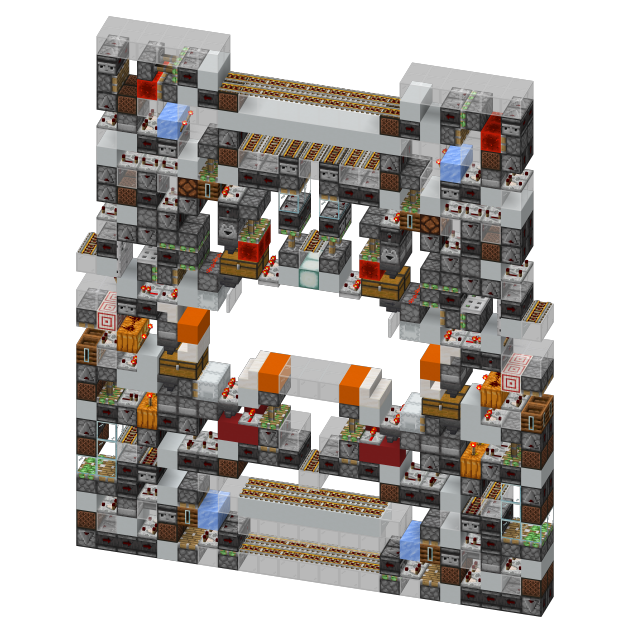
\includegraphics[width=0.48\textwidth]{slice.png}
    \caption{\centering DH02 Quad Display Slice}
\end{figure}

% For wide tables, a single column layout is better. It can be switched
% page-by-page.
\onecolumn

\section{Device Specifications}

\begin{table}[h]
    \caption{Device Specifications}
    \begin{tabularx}{\textwidth}{l | c c c | c | X}
        \thickhline
        \textbf{Parameter} & \textbf{Min.} & \textbf{Typ.} & \textbf{Max.} &
        \textbf{Unit} & \textbf{Conditions} \\
        \hline
        Item Throughput  & 8 & - & - & gt & Normal Usage \\
        \hline
        MC Version & 1.16 & 1.17.1 & - & MCV & Latest version at time of writing: 1.19.3\\
        \hline
        Dimensions & & 23 x 28 x 2 & & Blocks & \\
        \thickhline
\end{tabularx}
\end{table}
\newpage
\section{Testing Data}
\begin{table}[h]
\caption{Executed Tests}
\begin{tabularx}{\textwidth}{l | X}
    \thickhline
    \textbf{Test} & \textbf{Result} \\
    \hline
    Display operation & Box displays were able to replace boxes when emptied. \\
    \thickhline
\end{tabularx}
\end{table}

\section{Download Information}
\begin{table}[h]
    \caption{Download Information}
    \begin{tabularx}{\textwidth}{l | l | l | X}
        \thickhline
        \textbf{Identifier} & \textbf{MC} & \textbf{File} & \textbf{Description} \\
        \hline
        DH02 & 1.17.1 & \href{https://github.com/Soontech-Annals/Archive/blob/92d3541e07ddc3ab90360e923907f040eca76834/Archive/display-halls/DH02\%20Quad\%20Display\%20Slice\%20With\%20Passive\%20Read/DH02\_quadbulk\_slice\_2w\_dev1.litematic?raw=1}{DH02\_quadbulk\_slice\_2w\_dev1.litematic} & Litematic of slice. \\
        \hline
        \thickhline
    \end{tabularx}
\end{table}

\end{document}

